\documentclass{article}
\usepackage[utf8]{inputenc}
\usepackage{graphicx}
\usepackage{amsmath}
\usepackage{amssymb}
\usepackage{amsthm}
\usepackage{algorithm}
\usepackage{algorithmic}
\usepackage{biblatex}
\addbibresource{transfer_RL_survey.bib}

\graphicspath{{./images/}}


\title{TransferRL: Survey}
\author{Norio Kosaka}
\date{December 2018}

\begin{document}

\maketitle

\section{Profile of Paper}
\begin{itemize}
    \item Title: Transfer in Reinforcement Learning: a Framework and a Survey \cite{lazaric2012transfer}
    \item Author: Alessandro Lazaric
    \item Submitted Date: On 10 Jan 2013
\end{itemize}

\section{Content of Paper}
\begin{itemize}
    \item Introduction
    \item A Framework and a Taxonomy for Transfer in RL
    \begin{itemize}
        \item Transfer Framework
        \item Taxonomy
    \end{itemize}
    \item Methods for Transfer from Source to Target with a Fixed State-Action Space
    \begin{itemize}
        \item Problem Formulation
        \item Representation Transfer
        \item Parameter Transfer
    \end{itemize}
    \item Methods for Transfer across Tasks with a Fixed State-Action Space
    \begin{itemize}
        \item Problem Formulation
        \item Instance Transfer
        \item Representation Transfer
        \item Parameter Transfer
    \end{itemize}
    \item Methods for Transfer from Source to target Tasks with a Different State-Action Space
    \begin{itemize}
        \item Problem Formulation
        \item Instance Transfer
        \item Representation Transfer
        \item Parameter Transfer
    \end{itemize}
    \item Conclusions and Open Questions
\end{itemize}

\section{Abstract}
Transfer in RL is a relatively novel research area that focuses on transferring the knowledge from a set of source tasks to a target task to efficiently adapt the learning agent to it. In this present paper, they aim at providing a formalisation of the general transfer problem. First of all, I would like to define the word of \textit{Transfer} in learning procedure. A number of psychological studies (see e.g., Thorndike and Woodworth, 1901; Perkins et al, 1992) show that humans are able to learn a task better and faster by transferring the knowledge retained from solving similar tasks. Likewise, \textit{Transfer} in ML aims at designing the process that analyse the existing knowledge collected from a set of source tasks and transfer it so as to \textit{bias} the learning process on a target task towards a set of pre-defined \textit{good} hypotheses.

\section{Introduction}
\textbf{Transfer Learning in RL}: Transfer algorithms automatically build prior knowledge from the knowledge collected in solving a set of similar source tasks (i.e., \textit{training tasks}) and use it to bias the learning process on any new task (i.e., \textit{testing task}). And it normally results that a dramatic reduction in the number of samples for training stage and a huge improvement in the accuracy of on the target tasks.

\section{A Framework and a Taxonomy for Transfer in Reinforcement Learning}
\subsection{Transfer Framework}
We start off this section with looking at the fundamental notations regarding MDP, which is $\langle S_M, A_M, T_M, R_M \rangle$ where the state space, the action space, the transition function and the reward function, respectively. The \textit{space of tasks} involved in the transfer learning problems is denoted by $M = \{ M \}$. Let $\Omega$ be a probability distribution over the space of tasks $M$, finally we have the comprehensive notation representing the \textit{environment} $\epsilon = \langle M, \Omega \rangle$, which defines the setting of the transfer problem.

A standard learning algorithms take as input some form of knowledge of the task, denoted by $K$, and return a solution in a set of possible results, denoted by $H$. In this context, $K$ consists of all the elements used in the learning algorithm, such as instances(e.g., samples), the \textit{representation} of the problem(e.g., set of options, set of features), and also \textit{parameters}.Notice that $K$ includes \textit{prior knowledge} provided by an expert. Hence, we can renovate the generic learning algorithm in the following way;
$$
A_{learn}: K \rightarrow H
$$ where $a_{learn}$ represents the learning algorithm.

Given the previous definition, we can now define the general shape of the transfer learning algorithms with additional notations. Let $L$ be the number of tasks drawn from $M$ according to the distribution $\Omega$ used as source tasks and $K^L_S$ be the knowledge collected from the $L$ source tasks and finally $K_t$ be the knowledge available from the target task. The transfer phase will look like;
\begin{gather}
A_{transfer}: K^L_S x K_t \rightarrow K_{transfer}\\
A_{learn}: K_{transfer} x K_t \rightarrow H    
\end{gather}

\subsection{Taxonomy}
In this section, we will look at the three different aspects of the transferring in RL problem.
\subsubsection{The Settings}
In the following we will distinguish among three different categories of transfer setting
\begin{itemize}
    \item Transfer from source task to target task with fixed domain: most of the early literature focused on the problem in which the domain is fixed and only two tasks are involved: a source task and a target task.
    \item Transfer across tasks with fixed domain: In this setting, tasks share the same domain and the algorithm takes as input the knowledge collected from a set of source tasks and use it to improve the performance in the target task.
    \item Transfer across tasks with different domain: tasks have a different domain, that is the y might have different state-action space.
\end{itemize}

\subsection{The Knowledge}
In this section, we will classify the possible knowledge transfer approaches into three major categories.

\begin{itemize}
    \item Instance Transfer: The simplest version off transfer learning algorithm is to collect the samples(episodes) from the source task and uses them to to build a solution for the target task at hand.
    \item Representation transfer: After learning on different tasks, transfer algorithms often perform an abstraction process which changes the representation of the task and of the solutions, such as reward functions.
    \item Parameter transfer: this type of algorithm has to change and adapt the parameters used in the source task and apply them to the target task
\end{itemize}

\subsection{The Objectives}
In this section, we will look at the method to evaluate approaches, and classify them into three main categories.

\begin{itemize}
    \item Learning speed improvement: it is about the reduction in the amount of the experience needed to learn the solution of the task at hand.
    \item Asymptotic improvement: The core concept is that the more accurate the approximation is, the better the generalisation at convergence. This objective is usually targeted by representation-transfer algorithms.
    \item Jumpstart improvement: This objective is about the efficient exploration and normally used by \textit{parameter-transfer} algorithms
\end{itemize}

\section{Methods for Transfer from Source to Target with a Fixed State-Action space}
In this section, we will consider the simplest setting in which \textit{transfer} occurs from one source task to a target task.

\subsection{Problem Formulation}
We will consider the setting where the environment consists of two MDPs, a \textit{source task} $M_s = \langle S, A, T_s, R_s \rangle$ and a \textit{target task} $M_t = \langle S, A, T_t, R_t \rangle$, sharing the same state-action space as follows. Hence, the environment $\Epsilon$ is defined by the task space, $M = \{ M_s, M_t \}$ and a task distribution $\Omega$ which simply returns $M_s$ as the first task and $M_t$ as second. In figure4, it describes the basic problem setting for our transfer learning environment in this present paper, and it is about the navigation problem where the agent should move from the regions marked with $S$ to the goal region marked as $G$. Indeed, in this problem setting, the agent can easily find the similarity between the tasks of source and target. Then it is expected to apply the learning outcomes from the \textit{source task} to the \textit{target task}. 

\begin{figure}[h]
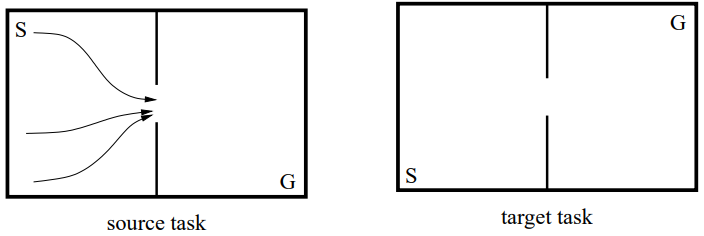
\includegraphics[width=\textwidth]{fig4}
\centering
\end{figure}

\subsection{Representation Transfer}
In representation transfer, it abstracts characteristic of the task from the source task. Then it changes the representation collected from the source task either of the solution space $H$ or of the MDP so as to speed-up the learning process in the target task. So, in this section, I would like to describe three different methods as follows;

\begin{itemize}
    \item Option Discovery: is to change the representation of the MDP by adding \textit{options} to the set of available actions.(Sutton et al., 1999 \cite{sutton1999between}) The core idea is to exploit the structure of the dynamics shared by the two tasks and to ignore the details in the specific source reward function. There are other approaches as well, \cite{mcgovern2001automatic} \cite{menache2002q}
    \item Action Space Transfer: using random task perturbation, a set of task is artificially generated from one single source task and the actions which end up with being not optimal are replaced with the generated actions. Then with the set of renewed actions, learning agent begins working on the target task. The advantage of this approach is that the reduction of unnecessary actions enhance the learning speed.(Sherstov and Stone, 2005\cite{sherstov2005improving}).
    \item Feature Discovery: this is sort of an advanced version of \textit{option discovery} in terms of exploring the similarity in characteristic between the source and target tasks. However, the biggest difference is that it extracts a set of features which defines the environment, instead of options and it is transferred to the target task from the one of source. Indeed, it does differ in terms of the purpose of the approach, for instance, \textit{Feature discovery} aims at achieving better approximation of the target value function. One of the approaches is that Mahadevan and Maggioni (2007)\cite{mahadevan2007proto} has proposed a method to generate \textit{proto-value functions} using spectral analysis of the \textit{Laplacian} of the estimated graph of the source MDP.
\end{itemize}

\subsection{Parameter transfer}
Previously stated approaches implicitly assumed the similarity of source and target tasks. Ferns et al (2004) and Phillips (2006) have examined the option-transfer approach to see if it can accommodate \textit{partially similar} target task. And they have come up with the metric to calculate the similarity of the environmental setting of the tasks, which is denoted as follows:
\begin{gather}
    d(s) = max_{a \in A}(|R_s(s,a) - R_t(s,a)| + \gamma J(d)(T_s(\cdot|s,a), T_t(\cdot|s,a)))
\end{gather} where $J(d)$ is the Kantorovish distance which measures the difference between the two transition distributions.

\section{Methods for Transfer across Tasks with a Fixed State-Action Space}
In previous section, we have considered the setting in which only one source task is available, in contrast, in this section we will review the main transfer approaches to the general setting when a set of source tasks is available. In this case, there are two things mattering.
\begin{enumerate}
    \item How to merge knowledge coming from different sources
    \item How to avoid the transfer from sources which differ too much from the target task
\end{enumerate}

\subsection{Problem Formulation}
In this section, we consider the setting in which the environment is defined by a set of tasks and a distribution. In fact, we can still assume that all the tasks share the same state-action space. But the reward functions do differ among tasks.

\subsection{Instance Transfer}
The core idea is that the transfer of source samples might improve the learning on the target task. For running example, we would like to consider the proposal of Lazaric et al (2008) \cite{lazaric2008transfer} which selectively transfers samples on the basis of the similarity between source and target tasks. As opposed to review earlier, this algorithm selects which source samples should be included in transfer batch based on a measure of similarity between the source and the target tasks. The number of source samples is assumed to be large enough to build an accurate kernel-based estimation of each source model. In the experiments reported in their research, this method is shown to successfully identify which sources are more relevant to transfer samples from and to avoid \textit{negative transfer}.

\subsection{Representation Transfer}
Unlike in the source-to-target transfer, the objective of representation transfer in this setting is to infer from the source tasks general characteristics that are preserved across the tasks and that can be effectively exploited to improve the average learning performance with respect to single-task learning.

\begin{itemize}
    \item Option Transfer: . Bernstein (1999) introduces a method to create a new option which is added to the set of available actions and which is built as a combination of the optimal policies learned on the L source tasks and it is then reused to speed-up learning process on the target task.
    \item Feature transfer to speed-up learning: it is to identify a function space which is likely to contain functions able either to speed-up the learning or to accurately approximate the optimal value functions. One particular method proposed earlier is to identify sub tasks and features according to the analysis of the dynamics of the source tasks, and solve them to find the optimal value-function.
    \item Feature transfer to improve asymptotic performance: While previously stated methods above are assuming the discrete MDPs, now we would like to consider the continuous state-action space in which function approximation is necessary. The objective is to learn the parameters which defines a feature space such that only a small set of features are used to approximate the value functions of the tasks.
\end{itemize}

\subsection{Parameter Transfer}
In contrast to representation-transfer approaches, all parameter-transfer algorithms explicitly define a distribution on the task space and try to estimate the true distribution in order to build a prior over the space of hypotheses so as to improve the initial performance and reduce the number of samples needed to solve any task in the distribution.

\begin{itemize}
    \item The hierarchical Bayesian Model: Using the representation of HBM, we can formulate the problem in the equation and solve it using \textit{Bayes Rule}.
    \item Inference for transfer: There is a simpler approach, which only uses the statistics about the action values. The mean and variance of the action values over different tasks are computed and then used to initialise the Q-table for new tasks.
\end{itemize}

\section{Methods for Transfer from Source to Target Tasks with a Different State-Action Spaces}
All the previous settings consider the case where all the tasks share the same \textit{domain}. In the most general transfer setting, however, the tasks may also differ in terms of number or range of the state-action variables.

\subsection{Problem Formulation}
In this section, we consider the case where the source task and target task have different MDPs respectively. And the approaches here can be summarised in three categories.

\begin{itemize}
    \item A hand-coded mapping
    \item learn a mapping from source to target
    \item extract from source task MDP some \textit{abstract knowledge} that can be reused to solve the target task
\end{itemize} And in this section, we would like to assume the \textit{mountain car domain} game on our mind.

\subsection{Instance Transfer}
Taylor et al (2008a) study the transfer of samples by considering the case where there exists only one source task and no specific method for the selection of the samples is implemented.
 
\subsection{Representation Transfer}
A number of transfer algorithms deal with the problem, which is that options learned on the source task are defined as a mapping from specific state to action space and they cannot be used in a target task with different state-action variables, by considering abstract options that can be reused in different tasks. For instance, Ravindran and Barto (2003); Soni and Singh (2006) use the homomorphism framework to map tasks to a common abstract level.
 
\subsection{Parameter Transfer}
Most of the algorithms in this approach are based on the hand-coded mappings and investigate how the transfer of different sources of knowledge influence the performance on the target tasks.

\section{Conclusions and Open Questions}
Although it has been long time to investigate the junction of \textit{transfer learning} and reinforcement learning, there are still a lot of things to be clear in the future. And in this section, I would like to briefly list the open questions for further work.

\begin{itemize}
    \item Theoretical analysis of transfer algorithms: although experimental results have already showed the effectiveness of transfer learning in RL, recent research has explored the improvement of the performance in the multi-task learning the supervised learning paradigm under certain circumstances.
    \item Transfer learning for exploration: study of optimal exploration, trade-off between exploitation and exploration.
    \item Concept drift and continual learning: One of the fundamental assumptions of transfer learning is that a clear distinction between the tasks in \textit{M} is possible. However, some recent researches has explored the case where the tasks vary over the time, such as non-stationarity of the environment.
\end{itemize}

\medskip
\printbibliography

\end{document}
